\documentclass{jsarticle}
\usepackage{amsmath, smssymb, amsfonts}
\usepackage{newtxtext, newtxmath}
\usepackage{latexsym}
\usepackage{mathrsfs}
\usepackage{mathtools}
\usepackage{textcomp}
\usepackage{mathcomp}
\usepackage[dvipdfmx]{graphicx, xcolor}
\usepackage{float}
\usepackage{wrapfig}	% must be after float package.
\usepackage{subcaption}
\usepackage{booktabs}
\usepackage{url}
\usepackage{listings, jvlisting, color}

\definecolor{OliveGreen}{rgb}{0.0,0.6,0.0}
\definecolor{Orenge}{rgb}{0.89,0.55,0}
\definecolor{SkyBlue}{rgb}{0.28, 0.28, 0.95}
\lstset{
  language={C++}, % 言語の指定
  basicstyle={\ttfamily},
  identifierstyle={\small},
  commentstyle={\smallitshape},
  keywordstyle={\small\bfseries},
  ndkeywordstyle={\small},
  stringstyle={\small\ttfamily},
  frame={tb},
  breaklines=true,
  columns=[l]{fullflexible},
  numbers=left,
  xrightmargin=0zw,
  xleftmargin=3zw,
  numberstyle={\scriptsize},
  stepnumber=1,
  numbersep=1zw,
  lineskip=-0.5ex,
  keywordstyle={\color{SkyBlue}},     %キーワード(int, ifなど)の書体指定
  commentstyle={\color{OliveGreen}},  %注釈の書体
  stringstyle=\color{Orenge}          %文字列
}


\begin{document}

\title{ゼミ レポート 08}
\author{山田 朔也}
\maketitle

\section{本レポートについて}
本レポートは6月21日に行われたゼミにて出題された課題に対するレポートとなっている。枕木磁壁の磁化構造を計算することとなる。

\section{原理}
\subsection{枕木磁壁}
有限の大きさを持つPermalloy薄膜の磁化構造を考える。このとき、図\ref{fig01}に示す構造を持つ。
\begin{figure}[H]
	\centering
	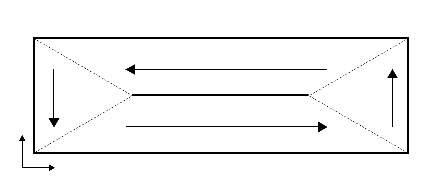
\includegraphics[width=14cm]{pic01.eps}
	\caption{Permalloy薄膜中の磁化構造(膜を上から見た図)}
	\label{fig01}
\end{figure}
膜の端の領域では、磁化が発生しないように磁気モーメントは境界に沿った方向を向く。
膜の内側では大きく4つの磁区構造と、それらを分ける3つの磁壁が現れる。
ここでは点線部の90度磁壁と、中心部の磁化ベクトルの向きが異なる$\mathrm{N\Acute{e}el}$磁壁が、
Bloch磁壁を挟んで交互に現れる磁壁構造の、二種に分けられる。

この枕木磁壁を計算する条件は、第2章第2節材料定数等の項に記載してあるものが適用される。

\subsection{静磁界計算}
第2章第2節材料定数等の項から、一つの計算点での静磁界は、計算領域内の全ての磁荷が作る静磁界の和となる。
すると、各計算セルの磁荷が観測点に作り出す磁界は式\ref{01}で表される。
\begin{align}
	Hx &= qxx\cdot mx + qxy\cdot my + qxz\cdot mz,	\notag \\
	Hy &= qxy\cdot mx + qyy\cdot my + qyz\cdot mz,	\label{01} \\
	Hz &= qxz\cdot mx + qyz\cdot my + qzz\cdot mz.	\notag 
\end{align}
ただし、$qxx,\,qyy,\,qzz,\,qxy,\,qxz,\,qyz$は静磁界係数とする。

静磁界係数は、各計算点と観測点の距離にのみ依存するため、第$\mathrm{(i,j)}$番目の計算点での静磁界は、式\ref{02}で表される。
\begin{align}
	Hx &= \sum_{i'=1}^{nx}\sum_{j'=1}^{ny}\left[ qxx(i'-i,j'-j)\cdot mx(i',j') + qxy(i'-i,j'-j)\cdot my(i',j') + qxz(i'-i,j'-j)\cdot mz(i',j') \right],	\notag \\
	Hy &= \sum_{i'=1}^{nx}\sum_{j'=1}^{ny}\left[ qxy(i'-i,j'-j)\cdot mx(i',j') + qyy(i'-i,j'-j)\cdot my(i',j') + qyz(i'-i,j'-j)\cdot mz(i',j') \right],	\label{02} \\
	Hz &= \sum_{i'=1}^{nx}\sum_{j'=1}^{ny}\left[ qxz(i'-i,j'-j)\cdot mx(i',j') + qyz(i'-i,j'-j)\cdot my(i',j') + qzz(i'-i,j'-j)\cdot mz(i',j') \right].	\notag 
\end{align}

今回の計算では上記の静磁界係数のうちいくつかは0になる。

\subsection{静磁界係数}
今回の静磁界係数の計算は、福島らによる論文[2]の手法を用いて計算を行う。

前回までの静磁界係数の算出方法では、立方体セルでの計算においては誤差が出なかった。
しかし、今回のような直方体セルの場合、セル内での静磁界に偏りが発生し、セル内の静磁界の平均値がセル中心での静磁界と一致しなくなる。
そのため、ここに誤差が現れるようになる。

これを解消するため、福島らによる論文[2]の手法を用いて、長方形セル内での静磁界の平均を取れるような静磁界係数を算出する。

\section{問題1}
\subsection{問題内容}
問題内容は、静磁界係数算出を行う事となる。
その上で以下の内容を調べる。
\begin{enumerate}
	\item 静磁界係数の対称性を調べる。
	\item 極端に偏平な計算セルを設定して静磁界係数を求め、qxx(0)は$-4\pi M$、それ以外は、ほぼ0の値になることを確認する。同様のことをqyy(0),qzz(0)についても調べる。
\end{enumerate}

\subsection{材料定数等}
材料定数等は、各小問の欄で特筆しない限り以下のものを使用する。
\begin{itemize}
	\item 計算点がx-y面に広がる2次元計算
	\item 直方体をセルを用いて離散化を行う
	\item 磁気モーメントを求める点は、各計算セルの中心に配置し、磁気モーメントは全て同じ方向を向くと仮定する。
	\item 飽和磁化$M = 800\;\mathrm{emu/cm^3}$
	\item 交換スティフネス定数$A = 1\times 10^{-6}\;\mathrm{erg/cm}$
	\item 異方性定数$K_u = 0\;\mathrm{erg/cm^3}$
	\item 損失定数$\alpha = 1$
	\item 磁気回転比$\lvert\gamma\rvert = 1.76\times 10^7\;\mathrm{rad/(s\cdot Oe)}$
	\item 時間刻み$\mathrm{dt} = 0.1\times 10^{-12}\;\mathrm{s}$
	\item 格子間隔$\mathrm{dx} = 80\;$\AA
	\item 格子間隔$\mathrm{dy} = 80\;$\AA
	\item 格子間隔$\mathrm{dz} = 450\;$\AA
	\item x方向の計算点数$\mathrm{nx} = 48$
	\item y方向の計算点数$\mathrm{ny} = 16$
	\item z方向の計算点数$\mathrm{nz} = 1$
	\item 境界領域では、ノイマン条件を用いる。
	\item 初期値は計算領域の中心を中心として反時計回りの方向を向いている円形状を初期値とし、磁壁の中心部では磁化を多少+z方向に持ち上げておく。
		その様子は図\ref{fig04}として掲載する。
\end{itemize}
\begin{figure}[H]
	\centering
	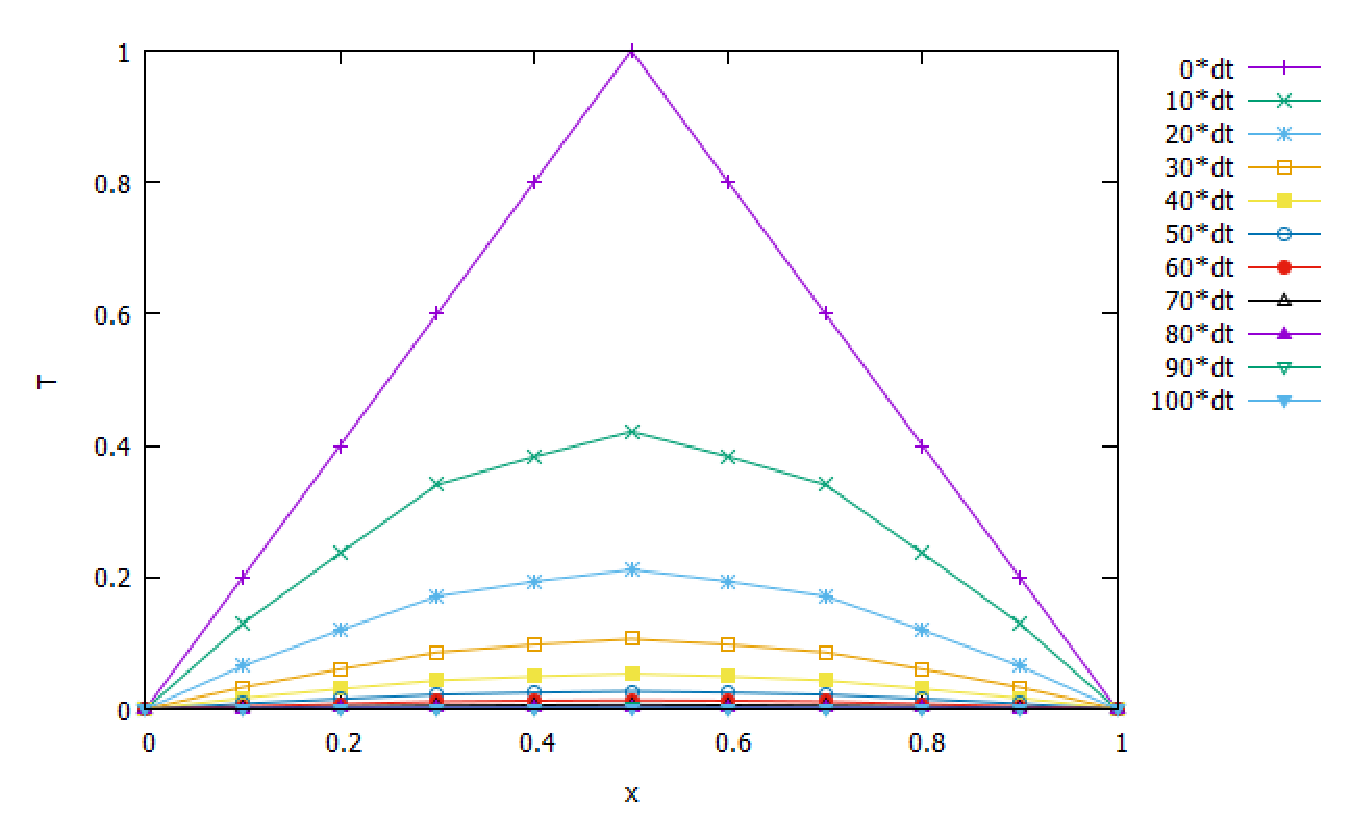
\includegraphics[width=14cm]{pic04.eps}
	\caption{磁化構造の初期値}
	\label{fig04}
\end{figure}

\subsection{小問1}
この問題では静磁界係数の対称性を調べる。

第2章第2節の材料定数を元に、qxx,\,qyy,\,qzz,\,qxy,\,qxz,\,qyzを計算した。
ただし、$\mathrm{nx} = 4,\,\mathrm{ny} = 2$とする。
その結果を図\ref{tab01}にまとめた。

\begin{figure}[H]
	\centering
	\begin{subfigure}{0.7\columnwidth}
		\centering
		\includegraphics[width=\columnwidth]{tab01_1.eps}
		\caption{qxxの計算結果}
		\label{tab01_1}
	\end{subfigure}
	\begin{subfigure}{0.7\columnwidth}
		\centering
		\includegraphics[width=\columnwidth]{tab01_2.eps}
		\caption{qyyの計算結果}
		\label{tab01_2}
	\end{subfigure}
	\begin{subfigure}{0.7\columnwidth}
		\centering
		\includegraphics[width=\columnwidth]{tab01_3.eps}
		\caption{qzzの計算結果}
		\label{tab01_3}
	\end{subfigure}
	\begin{subfigure}{0.7\columnwidth}
		\centering
		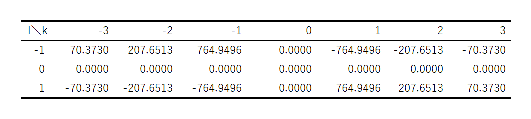
\includegraphics[width=\columnwidth]{tab01_4.eps}
		\caption{qxyの計算結果}
		\label{tab01_4}
	\end{subfigure}
	\begin{subfigure}{0.7\columnwidth}
		\centering
		\includegraphics[width=\columnwidth]{tab01_5.eps}
		\caption{qxzの計算結果}
		\label{tab01_5}
	\end{subfigure}
	\begin{subfigure}{0.7\columnwidth}
		\centering
		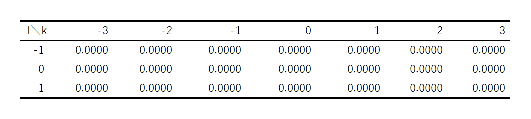
\includegraphics[width=\columnwidth]{tab01_6.eps}
		\caption{qyzの計算結果}
		\label{tab01_6}
	\end{subfigure}
	\caption{静磁界係数の計算結果}
	\label{tab01}
\end{figure}

図\ref{tab01_1},\,\ref{tab01_2},\,\ref{tab01_3}から、qxx,\,qyy,\,qzzは距離0を中心として、点対称の関係となっている。
図\ref{tab01_4}からは、qxyは距離0を中心として点対称だが、正負が入れ替わっていることが分かる。
また、x,yのいずれかの方向が0の場合は、qxyの値は0となることが分かる。
そして、図\ref{tab01_5},\,\ref{tab01_6}から、qxz,\,qyzの2つの係数は距離に関係なくほぼ0となる。

\subsection{小問2}
この問題では、極端に偏平な計算セルを設定して静磁界係数を求め、qxx(0)は$-4\pi M$、それ以外は、ほぼ0の値になることを確認する。

まずは計算条件について記述する。
qxx(0)を調べるときはdxを非常に小さくし、dy,\,dz非常に大きく設定する。($\mathrm{dx}=10$\,\AA$\mathrm{dy}=\mathrm{dz}=1\,\mathrm{cm}$)
これをqyy(0),\,qzz(0)も同様に、それぞれdy,\,dzを非常に小さくして計算する。
また、セル数を$\mathrm{nx}=4,\,\mathrm{ny}=2$とする。

このときの計算結果を図\ref{tab02}にまとめた。
\begin{figure}[H]
	\centering
	\begin{subfigure}{0.7\columnwidth}
		\centering
		\includegraphics[width=\columnwidth]{tab02_1.eps}
		\caption{qxxの計算結果}
		\label{tab02_1}
	\end{subfigure}
	\begin{subfigure}{0.7\columnwidth}
		\centering
		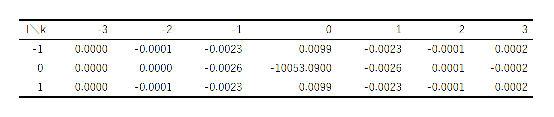
\includegraphics[width=\columnwidth]{tab02_2.eps}
		\caption{qyyの計算結果}
		\label{tab02_2}
	\end{subfigure}
	\begin{subfigure}{0.7\columnwidth}
		\centering
		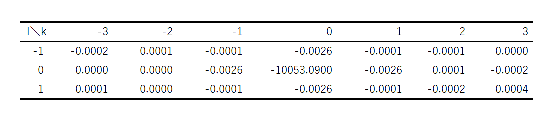
\includegraphics[width=\columnwidth]{tab02_3.eps}
		\caption{qzzの計算結果}
		\label{tab02_3}
	\end{subfigure}
	\caption{静磁界係数の計算結果}
	\label{tab02}
\end{figure}

ここで、$-4\pi M = 100053.0964915\cdots$なので、図\ref{tab02}のqxx(0),\,qyy(0),\,qzz(0)の値は、
想定していた値に非常に近い結果となった。
また、図\ref{tab02}から、中心点以外の点が0に近い値となっていることも分かる。

このことから、静磁界係数は正常に計算できていることが分かる。

\section{問題2}
\subsection{問題内容}
問題内容は、枕木磁壁の磁化構造を求めるプログラムを作成し、枕木磁壁の磁化構造を求める事となる。
また、動作が確認できたら、計算領域を拡張し大きな領域での構造を求める。

材料定数は第2章2節に準拠する。

\subsection{結果}
枕木磁壁の計算をした結果を図\ref{fig02}として示す。
\begin{figure}[H]
	\centering
	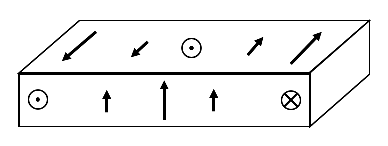
\includegraphics[width=14cm]{pic02.eps}
	\caption{枕木磁壁の磁化構造}
	\label{fig02}
\end{figure}

この図\ref{fig02}には、図\ref{fig01}で想定していた90度磁壁や、
$\mathrm{N\Acute{e}el}$磁壁がBloch磁壁を挟んで交互に現れる磁壁構造が、
存在している。
このことから、この計算結果が枕木磁壁であると分かる。

次に計算領域を拡張して計算した結果を図\ref{fig03}として示す。
\begin{figure}[H]
	\centering
	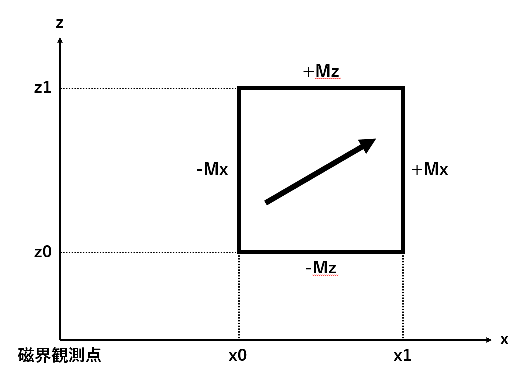
\includegraphics[width=14cm]{pic03.eps}
	\caption{拡張された枕木磁壁の磁化構造}
	\label{fig03}
\end{figure}

図\ref{fig03}から、領域を拡張すると枕木磁壁ではなく、Bloch磁壁になることが分かる。


\section{参考文献}

\begin{thebibliography}{9}
	\item 配布されたテキスト
	\item 
		H.Fukushima, Y.Nakatani, and N.Hayashi.
		\textit{Volume Average Demagnetizing Tensor of Rectangular Prisms}.
		IEEE Transactions on Magnetics, Vol.34, No.1, January 1998
\end{thebibliography}

\end{document}